\documentclass[]{article}

% text stuff
\usepackage{hyperref}
\usepackage[utf8]{inputenc}

% math stuff
\usepackage{amsmath}
\usepackage{amssymb}
\usepackage{amsfonts}
\usepackage{comment}

% diagram stuff
\usepackage{pgf}
\usepackage{tikz}
\usetikzlibrary{arrows, automata, positioning}

% code stuff
\usepackage{listings}
\usepackage{xcolor}

% quantum stuff
\usepackage{braket}

\definecolor{codegreen}{rgb}{0,0.6,0}
\definecolor{codegray}{rgb}{0.5,0.5,0.5}
\definecolor{codepurple}{rgb}{0.58,0,0.82}
\definecolor{backcolour}{rgb}{0.95,0.95,0.92}

\lstdefinestyle{mystyle}{
	backgroundcolor=\color{backcolour},   
	commentstyle=\color{codegreen},
	keywordstyle=\color{magenta},
	numberstyle=\tiny\color{codegray},
	stringstyle=\color{codepurple},
	basicstyle=\ttfamily\footnotesize,
	breakatwhitespace=false,         
	breaklines=true,                 
	captionpos=b,                    
	keepspaces=true,                 
	numbers=left,                    
	numbersep=5pt,                  
	showspaces=false,                
	showstringspaces=false,
	showtabs=false,                  
	tabsize=2
}

\lstset{style=mystyle}

% my stuff

% used wayyyy too common to not be a thing
% replaced by command in package braket
%\newcommand{\set}[1]{\left\{#1\right\}}
% block comment would be nice
%\newcommand{\comment}[1]{}
% Probability & expected value. Too bad somebody has taken \P
\newcommand{\Prob}[1]{\textbf{P}\left[#1\right]}
\newcommand{\Exp}[1]{\textbf{E}\left[#1\right]}
\newcommand{\Var}[1]{\textbf{Var}\left[#1\right]}
% Reals, Integers, etc
\newcommand{\N}{\mathbb{N}}
\newcommand{\R}{\mathbb{R}}
\newcommand{\Z}{\mathbb{Z}}
% Norms
\newcommand{\norm}[2][]{\lVert#2\rVert_{#1}}		
% dx, dy, etc.
\newcommand{\D}[1]{\mathop{d#1}}
% Fancy L for loss
\newcommand{\loss}{\mathcal{L}}
% Argmax, argmin, etc.
\DeclareMathOperator*{\argmax}{arg\,max}
\DeclareMathOperator*{\argmin}{arg\,min}
% Prevent fancy U+2212 minus signs from failing to register
\DeclareUnicodeCharacter{2212}{-}

%opening
\title{\vspace{-1in}CS 311 Programming Assignment 2}
\author{CS 311 Staff}

\begin{document}
\begin{center}
{\Large \bf COMPSCI 311 - Fall 2022}\\\
{\Large \bf PROG ASSGN 1: The Atomic Nature of Matter}
\end{center}
\noindent{\large \bf Due date: Friday, December 9th  at 11.59 PM EST}

\noindent

\section{Historical Perspective}

The atom played a central role in 20th century physics and chemistry, but prior to 1908 the reality of atoms and molecules was not universally accepted. In 1827, the botanist Robert Brown observed the random erratic motion of microscopic particles suspended within the vacuoles of pollen grains. This motion would later become known as Brownian motion. Einstein hypothesized that this motion was the result of millions of even smaller particles—atoms and molecules—colliding with the larger particles.

In one of his "miraculous year" (1905) papers, Einstein formulated a quantitative theory of Brownian motion in an attempt to justify the "existence of atoms of definite finite size." His theory provided experimentalists with a method to count molecules with an ordinary microscope by observing their collective effect on a larger immersed particle. In 1908 Jean Baptiste Perrin used the recently invented ultramicroscope to experimentally validate Einstein's kinetic theory of Brownian motion, thereby providing the first direct evidence supporting the atomic nature of matter. His experiment also provided one of the earliest estimates of Avogadro's number. For this work, Perrin won the 1926 Nobel Prize in physics.

\section{The Problem}

 In this assignment, you will redo a version of Perrin's experiment. Your job is greatly simplified because with modern video and computer technology—in conjunction with your programming skills—it is possible to accurately measure and track the motion of an immersed particle undergoing Brownian motion. We supply video microscopy data of polystyrene spheres ("beads") suspended in water, undergoing Brownian motion. Your task is to write a program to analyze this data, determine how much each bead moves between observations, fit this data to Einstein's model, and estimate Avogadro's number. This programming assignment was originally designed at the Princeton University \cite{PrincetonAvogadroAssignment}.

\section{Data}
We provide dataset obtained by William Ryu using fluorescent imaging. The dataset is stored in a subdirectory (named run\_1) and contains a sequence of two hundred 640-by-480 color images (named frame00000.jpg through frame00199.jpg). Here is a movie \href{https://www.cs.princeton.edu/courses/archive/spring17/cos126/assignments/atomic-files/atomic.mov}{mov} an motion. Figure \ref{fig:beads} is a typical raw image (left) and a cleaned up version (right) using thresholding, as described below.

\begin{figure}[h]
    \hfill%
	\scalebox{0.4}{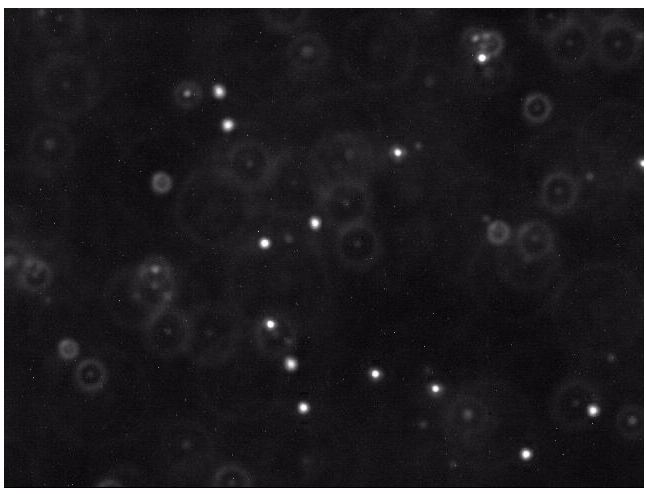
\includegraphics{fig1.png}}
    \hfill%
    \hfill%
    \hfill%
    \hfill%
    \hfill%
    \hfill%
    \hfill%
    \hfill%
    \hfill%
	\scalebox{0.4}{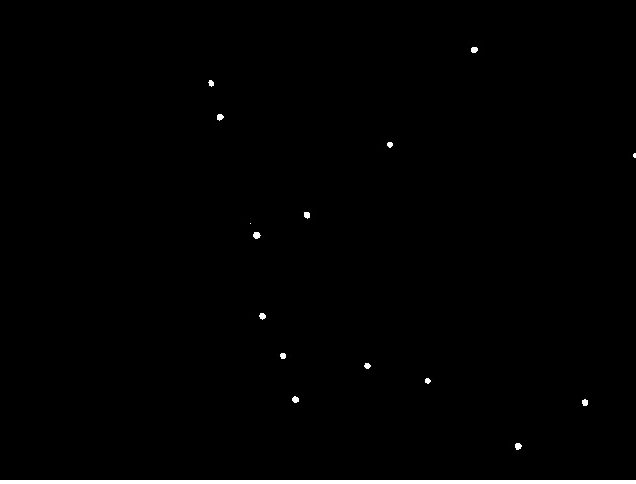
\includegraphics{fig2.png}}
	\caption{Image processed by the seam-carving algorithm. Note that the dimension of the image is reduced while the aspect ratio around important features on the image remains relatively unchanged.} \label{fig:beads}
    \hfill%
\end{figure}

Each image shows a two-dimensional cross section of a microscope slide. The beads move in and out of the microscope's field of view (the x- and y-directions). Beads also move in the z-direction, so they can move in and out of the microscope's depth of focus; this results in halos, and it can also result in beads completely disappearing from the image.

\section{Particle identification}
The first challenge is to identify the beads amidst the noisy data. Each image is 640-by-480 pixels, and each pixel is represented by a Color object which needs to be converted to a luminance value ranging from 0.0 (black) to 255.0 (white). Whiter pixels correspond to beads (foreground) and blacker pixels to water (background). We break the problem into three pieces: (i) read an image, (ii) classify the pixels as foreground or background, and (iii) find the disc-shaped clumps of foreground pixels that constitute each bead.

\subsection{Reading the image}
Use the Picture data type from Section 3.1 to read the image. By convention, pixels are measured from left-to-right (x-coordinate) and top-to-bottom (y-coordinate).

\subsection{Classifying the pixels as foreground or background}
We use a simple, but effective, technique known as thresholding to separate the pixels into foreground and background components: all pixels with monochrome luminance values strictly below some threshold tau are considered background; all others are considered foreground. The two pictures above illustrates the original frame (above left) and the same frame after thresholding (above right), using tau = 180.0.

\subsection{Finding the blobs}
A polystyrene bead is represented by a disc-like shape of at least some minimum number min (typically 25) of connected foreground pixels. A blob or connected component is a maximal set of connected foreground pixels, regardless of its shape or size. We will refer to any blob containing at least min pixels as a bead. The center of mass of a blob (or bead) is the average of the x- and y-coordinates of its constituent pixels.
We have created helper data type Blob that has the following API

\subsubsection{Python}
\begin{lstlisting}[language=Python]
    class Blob:
    """
    Represents a blob.
    """

    def __init__(self):
        """
        Constructs an empty blob.
        """
    def add(self, i, j):
        """
        Adds pixel (i, j) to this blob.
        """
    def mass(self):
        """
        Returns the number of pixels added to this blob, ie, its mass.
        """
    def distanceTo(self, other):
        """
        Returns the Euclidean distance between the center of mass of this blob
        and the center of mass of other blob.
        """
    def __str__(self):
        """
        Returns a string representation of this blob.
        """

\end{lstlisting}
Next, write a data type BlobFinder that has the following API. Use depth-first search to efficiently identify the blob. The API for python is below and the API for Java is in Section \ref{sec:Java:blobfinder}.
\begin{lstlisting}[language=Python]
    class BlobFinder:
    """
    A data type for identifying blobs in a picture.
    """

    def __init__(self, pic, tau):
        """
        Constructs a blob finder to find blobs in the picture pic, using a luminance threshold tau.
        """
    def _findBlob(self, pic, tau, i, j, marked, blob):
        """
        Identifies a blob using depth-first search. The parameters are the picture (pic), luminance threshold (tau), pixel column (i), pixel row (j), 2D boolean matrix (marked), and the blob being identified (blob).
        """
    def getBeads(self, P):
        """
        Returns a list of all beads with >= P pixels.
        """

\end{lstlisting}

 \subsubsection{Java} \label{sec:Java:blobfinder}
\begin{lstlisting}[language=Java]
public class Blob
-----------------------------------------------------------------
// constructed an empty blob
public Blob()        

// add a pixel (i, j) to the blob
public void add(int i, int j)  

// return number of pixels added = its mass
public int mass()   

// return distance between centers of masses of this blob and b
public double distanceTo(Blob b) 

// return string containing this blob's mass and center of mass
public String toString()         

// format center-of-mass coordinates with 4 digits to right of 
//decimal point
\end{lstlisting}

\begin{lstlisting}[language=Java]
public class BlobFinder
-----------------------------------------------------------------
// find all blobs in the picture using the luminance threshold tau
public BlobFinder(Picture picture, double tau)

// return the number of beads with >= P pixels
public int countBeads(int P)

// return all beads with >= P pixels
public Blob[] getBeads(int P)

\end{lstlisting}
\section{Particle tracking}
The next step is to determine how far a bead moves from one time t to the next time t + $\Delta t$. For our data, there are $\Delta t$ = 0.5 seconds between frames. Assume the data is such that each bead moves a relatively small amount and that beads never collide with one another. (You must, however, account for the possibility that the bead disappears from the frame, either by departing the microscope's field of view in the x- or y- direction, or moving out of the microscope's depth of focus in the z-direction.) Thus, for each bead at time t + $\Delta t$, calculate the closest bead at time t (in Euclidean distance) and identify these two as the same bead. However, if the distance is too large—greater than delta pixels—assume that one of the beads has either just begun or ended its journey.

\subsubsection{Python}
\begin{lstlisting}[language=Python]
def trackBeads(P, tau, delta, bf,image):
    return list
\end{lstlisting}

\subsubsection{Java}
\begin{lstlisting}[language=Java]
public class BeadTracker 
{
    public List<Double> BeadTrack(int P, double tau, double delta, String[] image) 
    {
    }
}
\end{lstlisting}

Complete the above given class in BeadTracker.java (bead\_tracker.py if you are coding in Python) that takes an integer min, a double value tau, a double value delta, and a sequence of image filenames as arguments; identifies the beads (using the specified values for min and tau) in each image (using BeadFinder); and returns the distance that each bead moves from one frame to the next (assuming that distance is no longer than delta) in form of list. You will do this for beads in each pair of consecutive frames, appending each distance that you discover, one after the other. Note that you must return a single list that will contain all the computed displacements across all consecutive images.

\section{Data analysis}
Einstein's theory of Brownian motion connects microscopic properties (e.g., radius, diffusivity) of the beads to macroscopic properties (e.g., temperature, viscosity) of the fluid in which the beads are immersed. This amazing theory enables us to estimate Avogadro's number with an ordinary microscope by observing the collective effect of millions of water molecules on the beads.
 
 \subsection{Estimating the self-diffusion constant}
 The self-diffusion constant D characterizes the stochastic movement of a molecule (bead) through a homogeneous medium (the water molecules) as a result of random thermal energy. The Einstein-Smoluchowski equation states that the random displacement of a bead in one dimension has a Gaussian distribution with mean zero and variance $\sigma^2 = 2 D \Delta t$, where $\Delta t$ is the time interval between position measurements. That is, a molecule's mean displacement is zero and its mean square displacement is proportional to the elapsed time between measurements, with the constant of proportionality 2D. We estimate $\sigma^2$ by computing the variance of all observed bead displacements in the x and y directions. Let ($\Delta x1, \Delta y1), ..., (\Delta xn, \Delta yn$) be the n bead displacements, and let $r_1, ..., r_n$ denote the radial displacements. Then

 \begin{equation}
     \sigma^2= \frac{(\Delta x_1^2+...... +\Delta x_n^2) + (\Delta y_1^2+....+\Delta y_n^2)}{2n}
     = \frac{r_1^2+....+r_2^2}{2n}
 \end{equation}

 For our data, $\Delta t = 0.5$ so this is an estimate for D as well. The radial displacements $r_i$ are measured in pixels: to convert to meters, multiply by $0.175 * 10^-6$ (meters per pixel).

\subsection{Estimating the Boltzmann constant}
 The Stokes-Einstein relation asserts that the self-diffusion constant of a spherical particle immersed in a fluid is given by

\begin{equation}
    D=\frac{kT}{6\pi\eta\rho}
\end{equation}
 where, for our data,
 
$T$ = absolute temperature = 297 degrees Kelvin (room temperature)

$\eta$ = viscosity of water = 9.135 * 10-4 N*s/$m^2$ (at room temperature)

$\rho$ = radius of bead = 0.5 * 10-6 meters 

and $k$ is the Boltzmann constant. All parameters are given in SI units. The Boltzmann constant is a fundamental physical constant that relates the average kinetic energy of a molecule to its temperature. We estimate k by measuring all of the parameters in the Stokes-Einstein equation, and solving for k.

 \subsection{Estimating Avogadro's number}
 Avogadro's number NA is defined to be the number of particles in a mole. By definition, $k = R / NA$, where the universal gas constant R is approximately 8.31457 J $K^{-1}$ $mol^{-1}$. Use $R / k$ as an estimate of Avogadro's number.
 
 \subsubsection{Python}
\begin{lstlisting}[language=Python]
def findAvogadroConstant(displacements):
    return k, N_A
\end{lstlisting}

 \subsubsection{Java}
\begin{lstlisting}[language=Java]
public class Avogadro 
{
    public List<Double> FindAvogadro(double [] rArray) 
    {
        
    }
}
    
\end{lstlisting}

\section{Code guidelines}

Here are the steps to follow:

\begin{itemize}

\item Download student\_submission folder from the resources tab on Piazza.

\item Run setup.sh to install required libraries.

\item For python, edit files blob\_finder.py, bead\_tracker.py and avogadro.py. 

\item For java, edit files BlobFinder.java, BeadTracker.java and Avogadro.java. Use compile.sh to compile your java files. To test locally, run java files using following command:

\begin{lstlisting}
    java -classpath "lib/*:." yourjavafile.java
\end{lstlisting}

\item Submission instructions. For Python, submit the files blob\_finder.py, bead\_tracker.py and avogadro.py to autograder. For Java, submit the files BlobFinder.java, BeadTracker.java and Avogadro.java.

\end{itemize}

%\section{References}

\bibliographystyle{unsrt}
\bibliography{library}

\end{document}
